\chapter{Modell}
\label{chp:Modell}

Im ersten Schritt soll die digitale Modellierung des zu erschaffenden Mars Rovers erfolgen.
Dazu wird gemäß der Spezifikation die Anwendung BrickLink-Studio (in der Version 2.0.10) genutzt.
Diese ermöglicht die umfangreiche und präzise Modellierung mit LEGO-Elementen sowie beispielsweise Funktionen zur Stabilitätsanalyse und Generierung schrittweiser Bauanleitungen.
In den folgenden drei Abschnitten sind jeweils eine gerenderte Front- und Seitenansicht und eine Draufsicht des Mars-Rover-Modells dargestellt.
Zusätzlich ist zum Vergleich in jedem Abschnitt eine Fotografie des realen Modells aus der entsprechenden Perspektive abgebildet.

\section{Vorderansicht}
\label{sec:voderansicht}

% TODO Vorderansicht render 
% TODO Vorderansicht foto

\begin{figure}
	\centering
	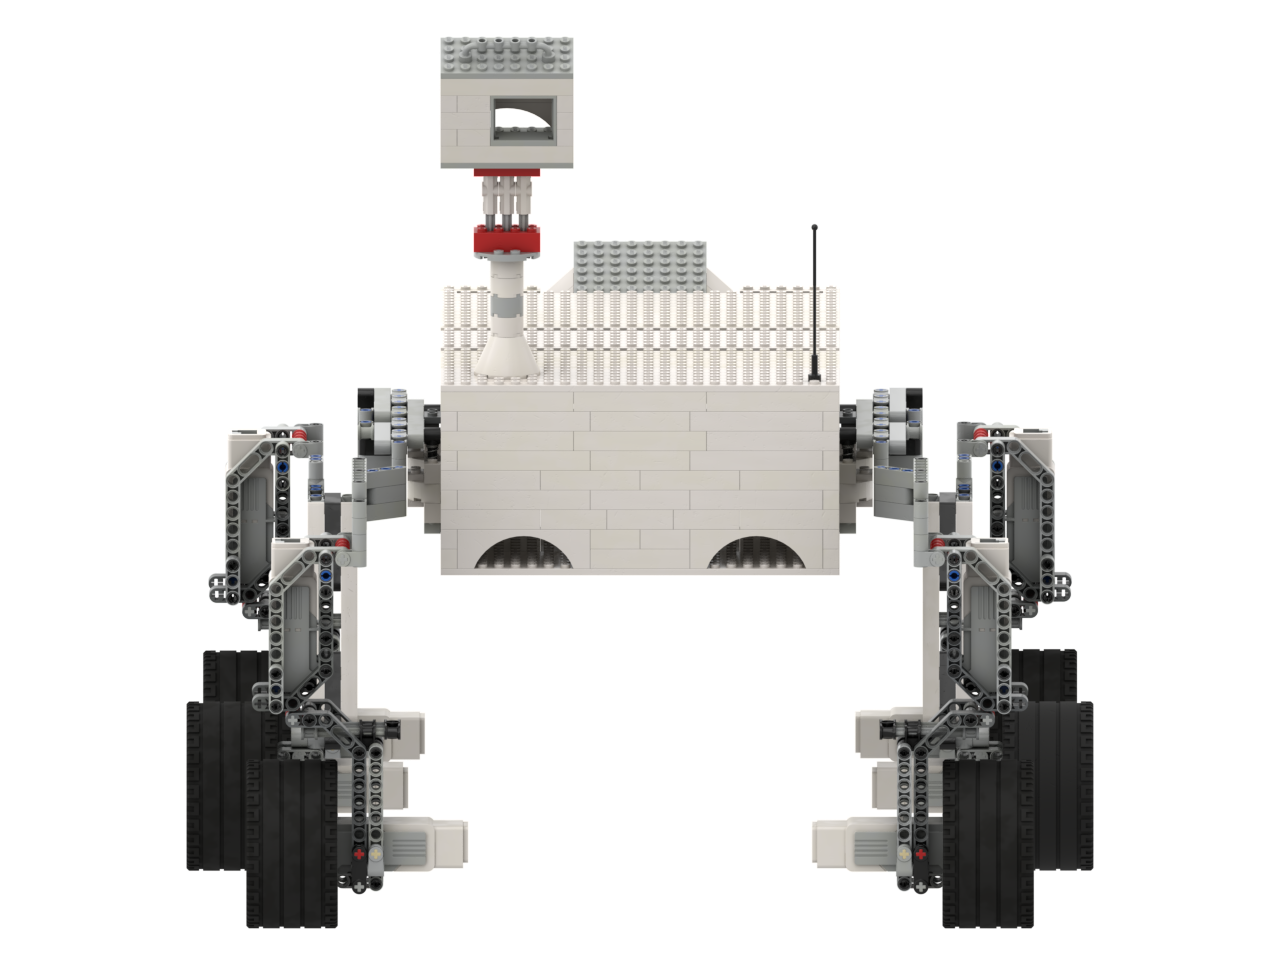
\includegraphics[width=0.8\textwidth]{../Images/Mars_Rover_V5_front.png}
	\vspace{0.5em}
	\parbox[c]{0.8\linewidth}{\footnotesize
		\centering
		\vspace{1em}
		Quelle: eigene Darstellung
	}
	\caption{Zusammenfassung der Aufgaben eines Datenbankkontextes im Entity Framework}
	\label{fig:dbcontext}
\end{figure}

\begin{figure}
	\centering
	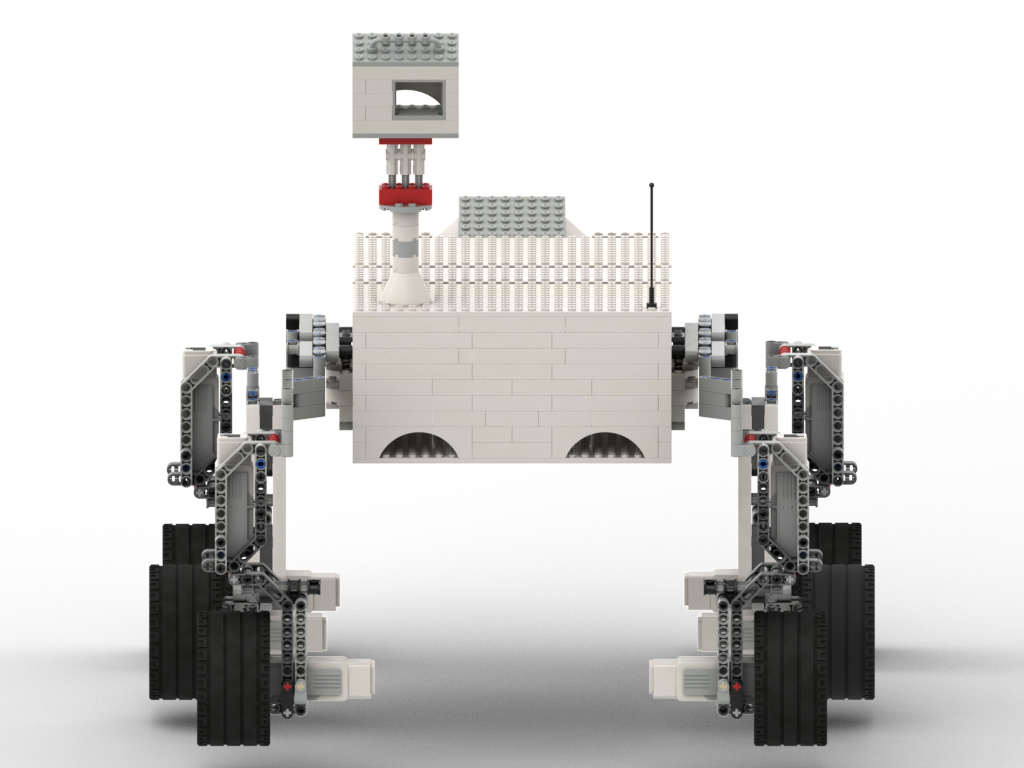
\includegraphics[width=0.8\textwidth]{../Images/Mars_Rover_V5_front_shadow.png}
	\vspace{0.5em}
	\parbox[c]{0.8\linewidth}{\footnotesize
		\centering
		\vspace{1em}
		Quelle: eigene Darstellung
	}
	\caption{Zusammenfassung der Aufgaben eines Datenbankkontextes im Entity Framework}
	\label{fig:dbcontext2}
\end{figure}

In der Frontalansicht erkennt man gut die zwei breiten Vorderräder, die über jeweils einen Motor zum Antrieb und einen für die Lenkung des Rades verfügen.
Über eine Aufhängung sind sie mit dem Korpus des Rovers verbunden und etwas von diesem abgesetzt, um die Stabilität zu erhöhen.
Weiterhin ist in der Realaufnahme die genutzte Kamera (siehe dazu Abschnitt \ref{sec:inst_konf_kamera}), platziert im charakteristischen Kopf des Rovers, erkennbar.
Der Kopf ist um $22{,}5 \degree$ nach unten geneigt, sodass die Erkennung von Wasserobjekten auch auf kurze Distanz möglich bleibt.

\section{Seitenansicht}
\label{sec:seitenansicht}

Der im vorherigen Abschnitt beschriebene Neigungswinkel des Kopfes wird in der Seitenansicht deutlich.
Weiterhin sind die mittleren und die Hinterräder des Rovers zu sehen.
Auf beiden Seiten sind diese starr miteinander verbunden und gemeinsam an einem einzigen Punkt mit einer vom Korpus ausgehenden, gefederten Strebe verbunden.
Dies entspricht dem Aufbau des Rocker-Bogie-Systems, welches bei \textit{Curiosity} zum Einsatz gekommen ist.
So ist sichergestellt, dass die mittleren Räder, die den Rover seitlich stabilisieren und antreiben, sowie die hinteren Räder, die ihn antreiben und gegebenenfalls lenken, in jedem Fall den Bodenkontakt beibehalten.
Bezüglich der Verbindung zum Korpus wurde vom Rocker-Bogie-System insofern abgewichen, dass dieser nicht frei um einen Punkt rotieren kann, da eine kontrollierte Verlagerung seines Schwerpunkts entlang der Fahrtrichtungsachse aktuell nicht ermöglicht werden kann.
Entsprechend besteht zum Beispiel durch Reibung an der Verbindungsstelle zur Aufhängung oder Windeinwirkung von vorn oder hinten die Gefahr, dass der Korpus kippt und nicht selbsttätig zurückgedreht werden kann.

\section{Ansicht von oben}
\label{sec:draufsicht}

Bei Betrachtung des realen Modells von oben erkennt man das Solarpaneel auf dem Korpus des Rovers.
Dieses soll die Energiegewinnung aus Sonnenlicht abbilden, wenngleich der Nennstrom des Moduls mit $250\ mA$ auf das Gesamtsystem keine großen Auswirkungen hätte.

Darüber hinaus ist hier ein guter Überblick über die Platzierung der einzelnen Räder und Motoren in Relation zum Korpus erkennbar.